\documentclass[10pt]{beamer}

\mode<presentation> 
{ \usetheme[nat,dogma]{Frederiksberg} }

% \usepackage[danish]{babel}
\usepackage[latin1]{inputenc}
\usepackage{times}
\usepackage[T1]{fontenc}
\usepackage[english]{babel}
\usepackage{hyperref}
\usepackage{animate}
%\usepackage{multimedia}
\usepackage{francois-preamble}
\usepackage{multirow}

\usepackage{multirow}
%\usepackage{movie15}

\newcommand{\cc}{{c\!\!,}}
\newcommand{\degr}[1]{{{#1}^\circ}}

\title{Vision and Image Processing: Optical Flow}

\author[F.~Lauze] % (optional, use only with lots of authors)
{Fran{\c c}ois Lauze}

\institute[DIKU] % (optional, but mostly needed)
{
  Department of Computer Science\\
  University of Copenhagen
}

\date[2015-2016 B2] % (optional, should be abbreviation of conference name)
% {Research Presentation, Diku 2006}

\definecolor{gold}{rgb}{0.95,0.83,0.0}
\definecolor{orange}{rgb}{0.95,0.7,0.0}
% \definecolor{backblue}{rgb}{0.93,0.94,0.99}
\definecolor{backblue}{rgb}{0.95,0.94,0.99}
\setbeamercolor*{background canvas}{bg=backblue} 



\newcommand{\myemph}[1]{{\color{blue}{#1}}}
\newcommand{\intrg}[1]{\int_{{#1}=-\infty}^\infty}
\newcommand{\intRR}{\int_{-\infty}^\infty}

\AtBeginSection[]
{
  \begin{frame}<beamer>{Outline}
    \tableofcontents[currentsection,currentsubsection]
  \end{frame}
}

\begin{document}
\maketitle

% would be cool with more images showing applications


%-------------------------------------------------------------------
%   Start slides
%-------------------------------------------------------------------




%----------------------------------------------



\begin{frame}
  \frametitle{Plan for today}
  \begin{itemize}
  \item Discuss a general introduction to True Motion and Apparent Motion.
  \item Discuss the Aperture Problem.
  \item Discuss approaches for apparent motion recovery.
  \item Present two old but still vigorous techniques: 
    \begin{itemize}
    \item Approach by Block-Matching
    \item Lucas and Kanade approach
    \item Horn and Schunck technique.
    \end{itemize}
  \item Discuss and reflect on some non-dense feature based techniques.
  \end{itemize}

\end{frame}




\section{Introduction}

\begin{frame}
  \frametitle{What is Optical Flow?}
  \begin{definition}{(From Wikipedia)}
    Optical flow or optic flow is the pattern of apparent motion of objects, surfaces, and
    edges in a visual scene caused by the relative motion between an observer (an eye or a
    camera) and the scene.
  \end{definition}
  \vfill\pause
  
  This raises questions about:
  \begin{itemize}
    \item image formation and projection of motion,
    \item link between projection of motion and observed patterns of apparent motions,
    \item and of course, how can it be recovered?
  \end{itemize}
\end{frame}

\begin{frame}
  \frametitle{An example}
  \begin{center}
    \includegraphics<1>{IMAGES/shr0}
    \includegraphics<2>{IMAGES/shr1}
    \begin{tabular}[h]{cc}
      \includegraphics<3>[width=0.4\textwidth]{IMAGES/shr0}& 
      \includegraphics<3>[width=0.4\textwidth]{IMAGES/shr1}\\
      \multicolumn{2}{c}{\includegraphics<3>[width=0.4\textwidth]{IMAGES/flowDavid}}
    \end{tabular}
  \end{center}
\end{frame}


\begin{frame}
  \frametitle{Applications of Optical Flow techniques}
 Applications are numerous e.g.\vfill
  \begin{itemize}
  \item Robotics -- robot navigation\vfill
  \item 3D scene understanding\vfill
  \item Surveillance\vfill
  \item Computer graphics and Augmented Reality\vfill
  \item Film restoration\vfill
  \item Motion compensation in Medical Images...
  \end{itemize}
\end{frame}





\section{Camera and Motion}

\begin{frame}
  \frametitle{Standard Pinhole Camera Model}
  \vfill
  \begin{center}
    \includegraphics[width=\textwidth]{FIGURES/standardpinholemodel}
  \end{center}
  \vfill
\end{frame}

\begin{frame}
  \frametitle{Alternative Pinhole Camera Model}
  \vfill
  \begin{center}
    \includegraphics[width=\textwidth]{FIGURES/pinholecamera_alt}
  \end{center}
  \vfill
\end{frame}


\begin{frame}
  \frametitle{Pinhole Camera Model I}
  \begin{center}
    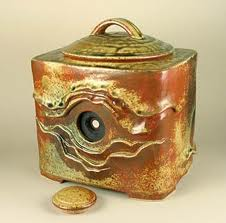
\includegraphics[width=\textwidth]{FIGURES/pinholecamera}
  \end{center}
\end{frame}

\begin{frame}
  \frametitle{Pinhole Camera Model II}
  The 2D to 1D case:
  \begin{center}
    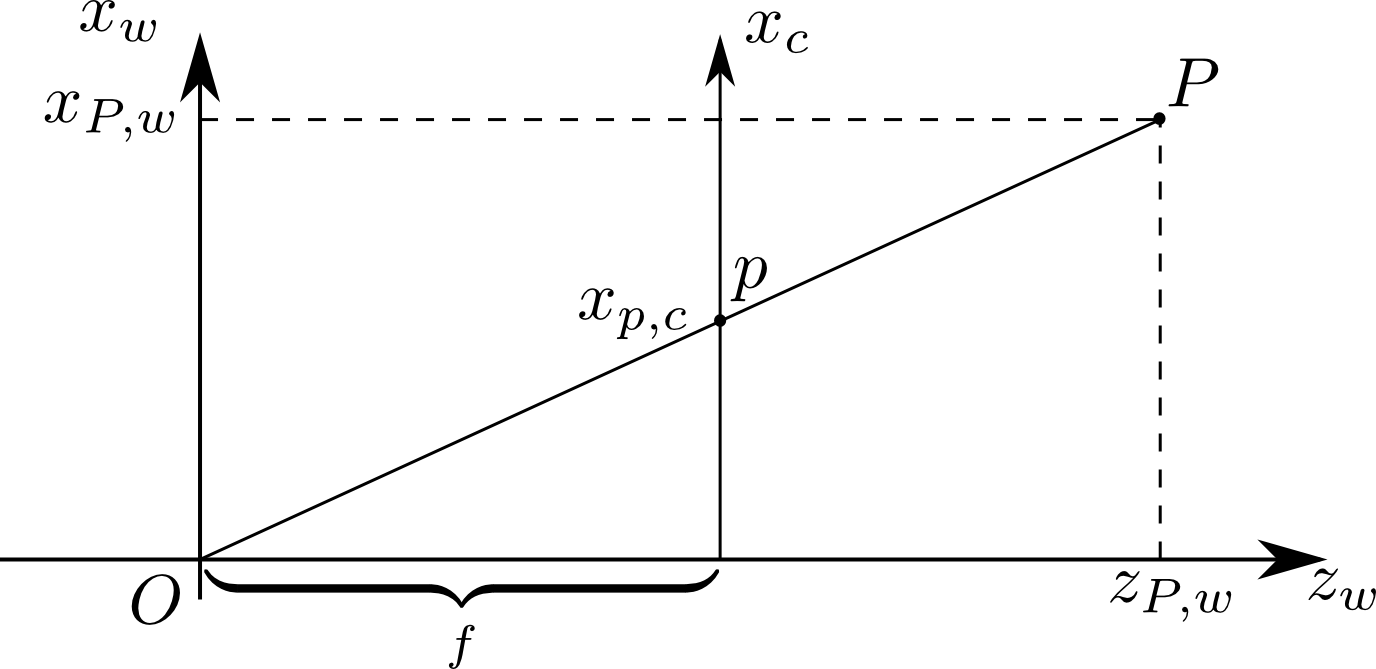
\includegraphics[width=0.75\textwidth]{FIGURES/pinholecamera1D}
  \end{center}
  $$
  \frac{x_{p,c}}{f} = \frac{x_{P,w}}{z_{P,w}}\quad\Iff x_{p,c} = f\frac{x_{P,w}}{z_{P,w}}
  $$
  \end{frame}

\begin{frame}
  \frametitle{Projection Onto Camera Plane}
  \begin{itemize}
  \item 3D to 2D projection.
    $$
    P_w =
    \begin{pmatrix}
      x_w\\y_w\\z_w
    \end{pmatrix}
    \quad\Implies\quad
    P_c =\frac{f}{z_w}
    \begin{pmatrix}
      x_w\\y_w
    \end{pmatrix}
    $$
  \item With motion: need time!
    $$
    P_c(t) = \frac{f}{z_w(t)}
    \begin{pmatrix}
      x_w(t)\\y_w(t)
    \end{pmatrix}
    $$
  \end{itemize}
\end{frame}


\begin{frame}
  \frametitle{Pinhole Camera Model and Motion I}
  \begin{center}
    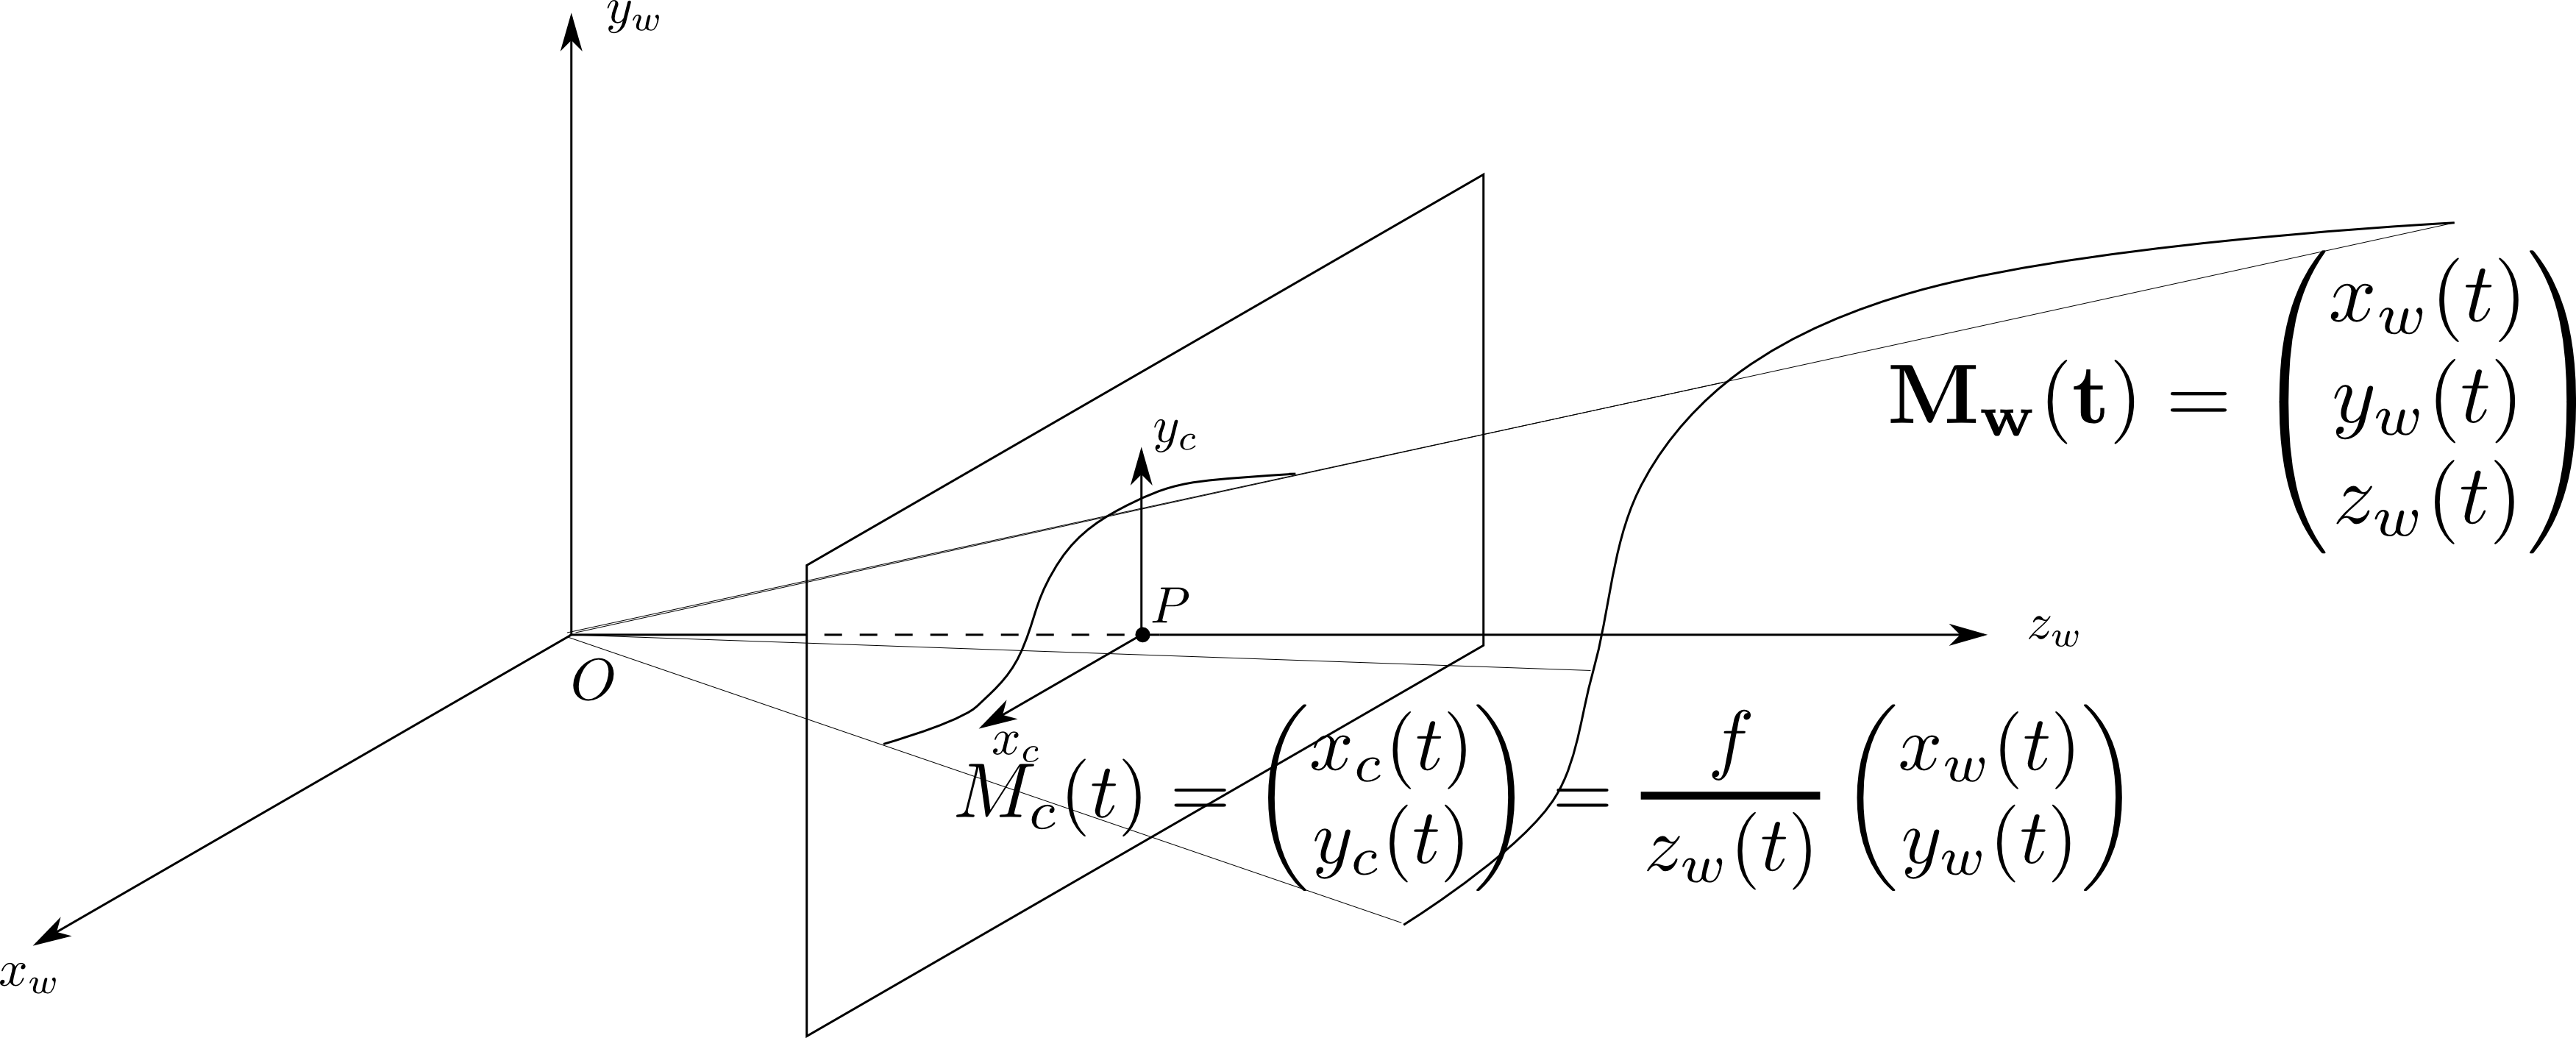
\includegraphics[width=\textwidth]{FIGURES/pinholecameramotion}
  \end{center}
  \begin{itemize}
  \item Motion in the ``world'' induces motion on the camera plane. But the relation is
    not simple, $z_w(t)$ in the denominator.
 
  \end{itemize}
\end{frame}



\begin{frame}
  \frametitle{Pinhole Camera Model and Motion II}
  \begin{itemize}
  \item If $z_w$ does not change, much easier, but it means that the motion trajectory is
    parallel to the camera plane.
  \item Two objects with same speeds, moving parallel to the $xy$-plane but with
    different $z$-values will show different apparent motion: the object farther to the
    camera plane appears to move slower: \myemph{motion parallax}.
    \begin{center}
      \includegraphics[width=0.75\textwidth]{FIGURES/pinholepara}
    \end{center}
  \item Other phenomena?
  \end{itemize}
\end{frame}

\begin{frame}
  \frametitle{True vs Apparent Motion}
  \begin{itemize}
  \item Apparent motion usually originates from true motion
  \item But there are ambiguities in apparent motion, e.g.,
  \item Motion parallax phenomenon or slower displacement of larger objects?
  \item Camera zooming in / out (or eq. object getting closer or
    farther from camera) vs. object changing size?
  \item Other image cues / perceptual a priori are used for disambiguation.
  \item But we can still be fooled -- and computers too.
  \end{itemize}
\end{frame}


\section{Apparent Motion}
\label{sec:appmot}

\begin{frame}
  \frametitle{Image Content Change and Apparent Motion}
  \begin{itemize}
  \item Motion is observed via image content change:\vfill
  \item If a punctual object projected at pixel $p$ moves with (projected) motion
    $\vec{v_p}$, it should be observed at pixel $p+\vec{v_p}$.\vfill
  \item Idea: A image dependent quantity $F(I)$ at position $p$ in first image should be
    observed at position $p+\vec{v_p}$ in the second image:
    $$
    F(I_1)(p) = F(I_2)(p+\vec{v_p})
    $$\vfill
  \end{itemize}
\end{frame}

\begin{frame}
  \frametitle{Displaced Frame Difference}
  \begin{itemize}
  \item Most usual choice: intensity of objects is preserved during motion:
    \begin{equation}
      \label{eq:dfde}
      I_1(p) = I_2(p+\vec{v_p})
    \end{equation}
  \item Only valid under limited illumination conditions -- the \myemph{Lambertian Model}.
  \item Equation \eqref{eq:dfde} sometimes called \myemph{Displaced Frame Difference Equation (DFDE)}
  \end{itemize}
  \begin{center}
    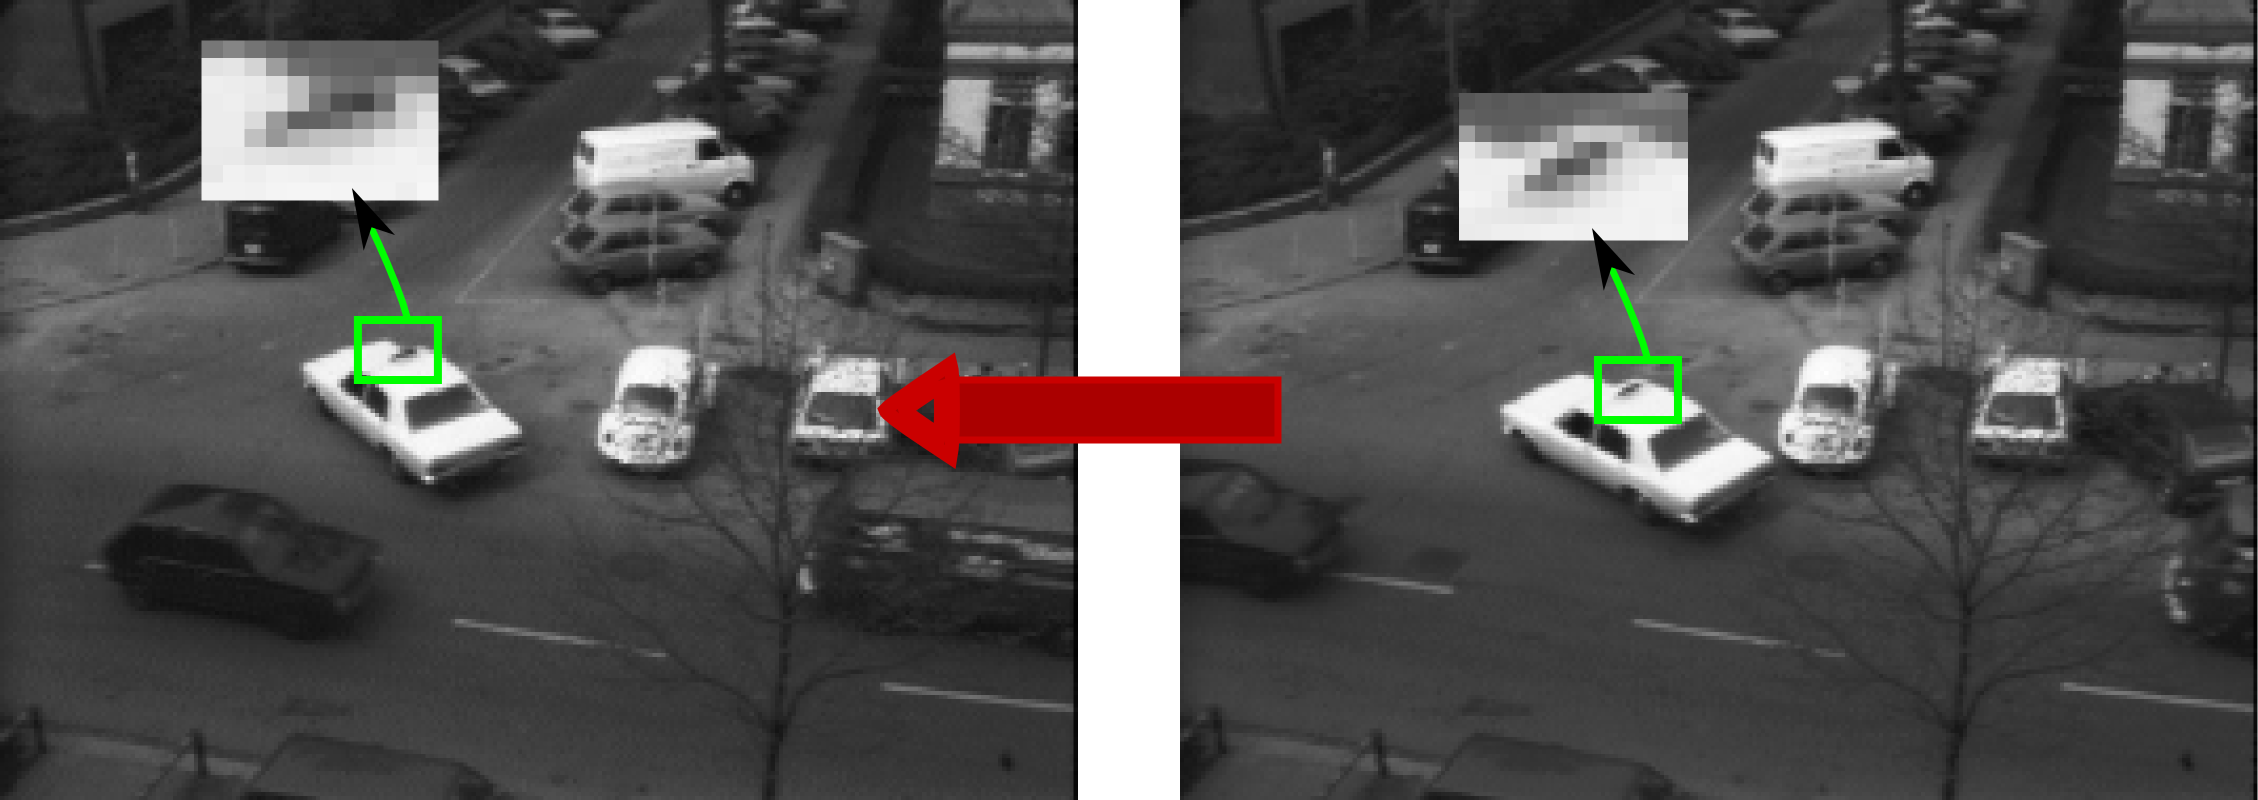
\includegraphics[width=0.8\textwidth]{FIGURES/taxiframemotion}
  \end{center}
\end{frame}




\begin{frame}
  \frametitle{Optical Flow Constraint Equation I}
  \begin{itemize}
  \item Apply Taylor formula to  Displaced Frame Difference Equation for $p=(x_0,y_0)$ and $\vec{v_p} = (v_{p1},v_{p2})^T$
    $$
    I_2(x_0 + v_{p1}, y_0 + v_{p2}) - I_1(x_0,y_0) = 0.
    $$
    $$
    \Downarrow
    $$
    \begin{align*}
      0 &= I_2(x_0 + v_{p1}, y_0 + v_{p2}) - I_1(x_0,y_0) \\
      &\simeq \nabla_{(x_0,y_0)} I_2\cdot \vec{v_p} + \udesc{I_t}{I_2(x_0,y_0)-I_1(x_0,y_0)}
    \end{align*}
  \item The quantity $I_t$ is the ``time-derivative'' of the observed
    moving image. Equation above is called the \myemph{Optical Flow
      Constraint Equation} for the pair of images $(I_1,I_2)$
  \end{itemize}
\end{frame}


\begin{frame}
  \frametitle{Optical Flow Constraint Equation II}
  \begin{itemize}
  \item Consider that $I_1$ and $I_2$ are the observations of the
    \myemph{Image Sequence} $I(x,y,t)$ between time $t_0$ and $t_1 =
    t_0 + dt$ ($dt$ small). 
  \item Above formula can be rewritten as
    $$
    I(p+\vec{v},t+dt) -I(p,t) \approx \nabla_{(p,t)} I\cdot (v_1,v_2,dt)^T \approx 0
    $$
  \item This is the \myemph{Optical Flow Constraint Equation (OFCE)}
    for Image sequence $I(-,-,t)$ for a small displacement $v_p$.
  \end{itemize}
\end{frame}


\begin{frame}
  \frametitle{Optical Flow Constraint Equation III}
  \begin{itemize}
  \item Image plane point $p$ moves: $p = p(t) = (x(t), y(t))$,  intensities along trajectory conserved.
    $$
    f(t) = I(p(t), t) = \text{constant}.
    $$
    Differentiate w.r.t. $t$
    $$
    f'(t) = \nabla_{(p,t)}I\cdot \uder{p}{t} + \pder{I}{t} = 0
    $$
    (Spatial gradient here, not spatio-temporal).  This is another of
    the commonly used forms of the OFCE.
  \item $dp/dt = $ \myemph{instantaneous velocity} at
    time $t$ (pixels per second) while $v_p$ from previous slide is a displacement (pixels).
  \end{itemize}
\end{frame}


\begin{frame}
  \frametitle{One-dimensional signals}
  \begin{center}
    \includegraphics[width=0.85\textwidth]{FIGURES/OFCE1D}
  \end{center}
  OFCE in 1D reads 
  $$
  \pder{I}{x}v + \pder{I}{t} = 0 \quad v = -\frac{I_t}{I_x}
  $$
   ($I_x$ alternate notation for $\pder{I}{x}$, idem for $t$)\\
   1 equation $\leftrightarrow$ 1 degree of freedom.
\end{frame}



\begin{frame}
  \frametitle{Aperture Problem}
  \begin{itemize}
  \item In dimension 2
    $$
    \pder{I}{x}v_1 +  \pder{I}{y}v_2 + \pder{I}{t} = 0
    $$
  \item 1 equations for 2 unknowns, , one extra degree of freedom! Punctual form of the \myemph{aperture problem}.
  \item Only the component of $\vec{v}$ parallel to $\nabla I$ can be computed
    $$
    \vec{v} = (v_1,v_2)^T = \alpha \frac{\nabla I}{|\nabla I|} + \beta\frac{\nabla I^\bot}{|\nabla I|}
    $$
    $$
    \alpha = -\frac{I_t}{|\nabla I|}
    $$
  \end{itemize}
\end{frame}


\begin{frame}
  \begin{center}
    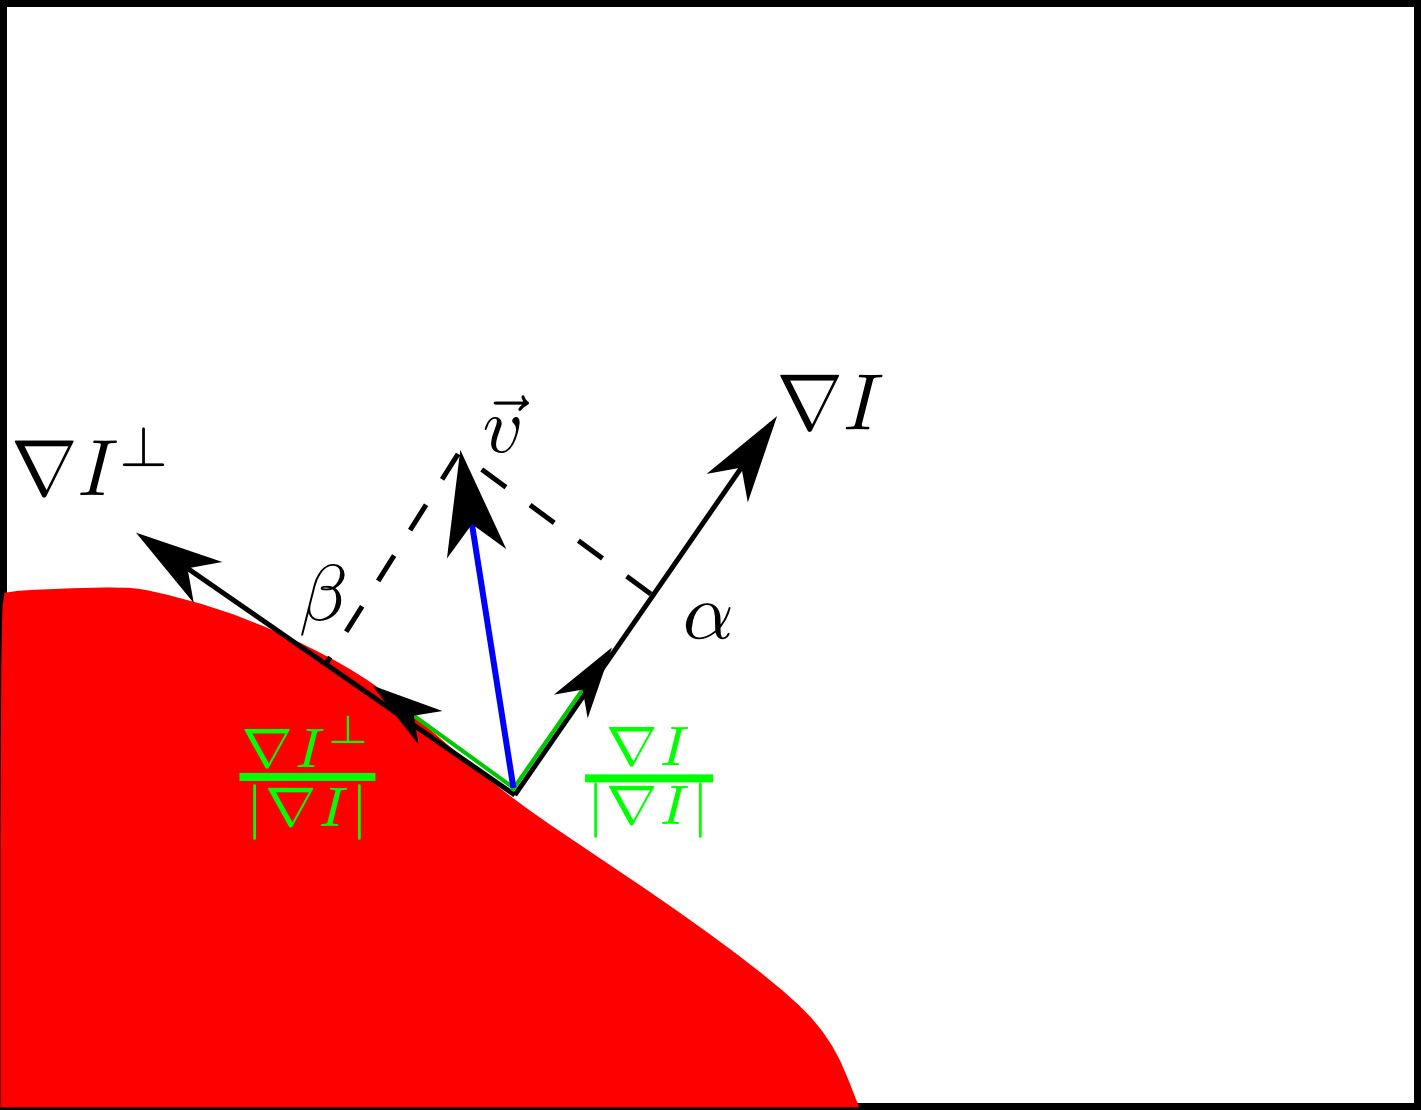
\includegraphics[width=0.75\textwidth]{FIGURES/optflownormal}
  \end{center}
\end{frame}


\begin{frame}
  \frametitle{Aperture Problem II}
  \begin{itemize}
  \item Perception of apparent motion depends on structures and their size:
  \end{itemize}
  \begin{center}
    \begin{tabular}[h]{cc}
      \includegraphics<1>[width=0.4\textwidth]{FIGURES/aperture1}
      \includegraphics<2->[width=0.4\textwidth]{FIGURES/aperture2}&
      \includegraphics<3>[width=0.4\textwidth]{FIGURES/aperture3}\\
      Moving bar structure & Apparent motion
    \end{tabular}
  \end{center}
\end{frame}


\begin{frame}
  \frametitle{Aperture Problem II}
  \begin{itemize}
  \item By ``increasing the aperture'', more visible structure:
  \end{itemize}
  \begin{center}
    \begin{tabular}[h]{cc}
      \includegraphics<1>[width=0.4\textwidth]{FIGURES/aperturecn1}
      \includegraphics<2->[width=0.4\textwidth]{FIGURES/aperturecn2}&
      \includegraphics<3>[width=0.4\textwidth]{FIGURES/aperturecn3}\\
      Moving corner structure & Apparent motion
    \end{tabular}
  \end{center}
\end{frame}


%%%%%%%%%%%%%%%%%%
%% A retravailler
%%%%%%%%%%%%%%%%%%
\begin{frame}
  \frametitle{Aperture Problem III}
  \begin{itemize}
  \item In the absence of other cues, the simplest motion is perceived:
    \begin{center}
      \includegraphics[width=0.8\textwidth]{FIGURES/aperture_simplest}
    \end{center}
  \item In this case, perceived motion is the shortest, and orthogonal to structure.
  \item But these two motion vectors are equally valid.  Their
    component orthogonal to the moving structure are \myemph{equal}
    and this is the component parallel to image gradient.
  \item Competition between cues and simplicity is part of optical flow algorithms.
  \end{itemize}
\end{frame}




\begin{frame}
  \frametitle{Wrong Motion Perception: The Barber Pole Illusion}
  \begin{columns}
  \column{0.5\textwidth}
  \begin{center}
    \animategraphics[loop,scale=0.5]{24}{IMAGES/bp/barberpole_frame_}{01}{24}
  \end{center}
  Pole is turning from right to left\\
  Perceived motion is upward!
  \column{0.5\textwidth}
  \begin{center}
    \includegraphics[width=0.65\textwidth]{FIGURES/barberpolemotion}
  \end{center}
  True and perceived motion
  \end{columns}
  
\end{frame}




\section{Optical Flow Recovery}
\label{sec:optrec}

\begin{frame}
  \frametitle{Important Principles Behind Recovery}
  \begin{itemize}
  \item Motion Coherence: pixels in an object of a scene move coherently:
    \begin{center}
      \includegraphics[width=0.65\textwidth]{FIGURES/pinholecameramotioncoherence}
    \end{center}
  \item Motions vectors also do not change too much with time:
    temporal coherence (less used).  
  \item Spatial coherence may solve the aperture problem.
  \end{itemize}
\end{frame}


\begin{frame}
  \frametitle{Occlusions and Disocclusions}
  \begin{itemize}
  \item Two or more objects moving in the scene at different depths
    and with  different motions . One may partially hide another:
    Motion discontinuity.
    \begin{center}
        \includegraphics[width=0.65\textwidth]{FIGURES/pinholecameramotionocclusion}
    \end{center}
  \item Using too large spatial coherence may use motions from
    different objects: need to find these boundaries. Usually
    are seen as image edges.
  \item But not all image edges are object boundaries. And some
    boundaries are not always clear.
  \end{itemize}
\end{frame}



\begin{frame}
  \frametitle{Noise, Measurement Errors and Other Disturbances}
  Neither the DFDE $I_2(x+v_1,y+v_2) - I_1(x,y) = 0$ nor the OFCE $I_x v_1 + I_y v_2 + I_t = 0$
    hold for most sequences / image pairs, even for ``exact'' motion vector $\vec{v} = (v_1,v_2)^T$.
    Several reasons For that:
 \begin{itemize}
  \item Noise alter pixel values:
  \item Subpixelic motion means partial pixel effects
  \item Change in lightning condition: no perfect Lambertian scenes
  \item Occlusion / disocclusion.
  \item Other reasons...?
  \end{itemize}
\end{frame}
\begin{frame}
  \frametitle{How to Deal With Them }
  \begin{itemize}
  \item Solution: use in \myemph{least-squares} settings: square-residual
    $$
    \left(I_2(x+v_1,y+v_2) - I_1(x,y)\right)^2
    $$
    should be as small as possible.
  \item Can also use absolute value residual
    $$
    |I_x v_1 + I_y v_2 + I_t|
    $$
    as small as possible (better for occlusion / disocclusion).
  \item Robust statistic approach too.
  \item We only consider least squares approaches here.
  \end{itemize}
\end{frame}



\begin{frame}
  \frametitle{Algorithms for Recovery}
  \begin{itemize}
  \item Many families of algorithms for motion recovery.\vfill
  \item Since 1980, more than 3000 papers!\vfill
  \item We briefly look at three ``grand old'' classical ones:\vfill
    \begin{enumerate}
    \item Block Matching.\vfill
    \item The Lucas and Kanade approach.\vfill
    \item The Horn and Schunck approach.
    \end{enumerate}
  \end{itemize}
\end{frame}

\begin{frame}
  \frametitle{Block Matching }
  \begin{itemize}
  \item A conceptually very simple algorithm, use patch matching.\vfill
  \item Matching patches can solve for the aperture problem (though patch size can be an issue).\vfill
  \item Not always very precise, has difficulties to capture complex motion behaviors.\vfill
  \item Very fast and a lot of variations exist.\vfill
  \item Used in video compression (behind many mpeg-type encoders).
  \end{itemize}
\end{frame}

\begin{frame}
  \begin{itemize}
  \item  Create a small block around 1 pixel in
    image $I_1$ Search for a similar block in image $I_2$ usually by
    minimizing sum of squares differences (SSD).
    \begin{center}
      \includegraphics[width=0.55\textwidth]{FIGURES/blockmatch}
    \end{center}\vfill
  \item ``Kernel'' block of size $s\times s$ ($s$ usually odd, $s = 2k+1$ with block centered around pixel $p = (x,y)$)
  \end{itemize}
\end{frame}  

\begin{frame}
  \begin{itemize}
  \item Search window of size $(2\ell +1)\times(2\ell+1)$ (provides
    max displacement allowed) in image 2 centered at position
    $(x,y)$.\vfill
  \item
    With odd size kernel size $2k+1$,  score to minimize:
    \begin{align*}
      m_{v_1,v_2} &= \sum_{i=-k}^k\sum_{j=-k}^k\left(I_1(x+i,y+j)- I_2(x+i+v_1,y+j+v_2)\right)^2\\
      v_1 &= -\ell\dots\ell,\quad v_2 = -\ell\dots\ell
    \end{align*}
  \end{itemize}
\end{frame}


\begin{frame}
  \begin{itemize}
  \item Minimizing above score very similar to maximizing the correlation between patches.
  \item Given by
    $$
    c(v_1,v_2) = \sum_{i=-k}^k\sum_{j=-k}^k I_1(x+i,y+j)I_2(x+i+v_1,y+j+v_2)
    $$
  \item This a dot product between a fixed patch and a moving one!
  \item Normalize correlation could be used instead -- provides the
    cosine of the angles between the fixed patch in image $I_1$ and
    the moving patch in image $I_2$.
  \item Correlation can be implemented fast using Fast Fourier Transform.
  \end{itemize}
\end{frame}


\begin{frame}
   \begin{itemize}
   \item Large displacements means a large search space ($\ell >> 0$)
   \item It can be reduced by a pyramid search approach (smoothing and downsampling)
     \begin{center}
       \begin{tabular}[h]{cc}
         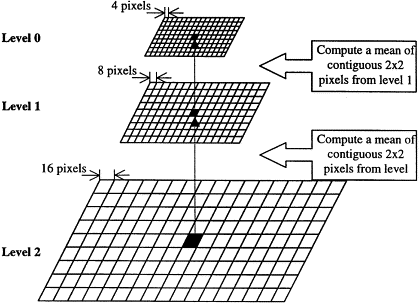
\includegraphics[width=0.45\textwidth]{FIGURES/bmpyramid1}&
         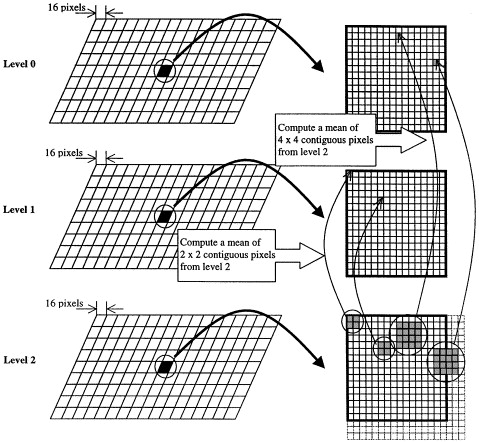
\includegraphics[width=0.45\textwidth]{FIGURES/bmpyramid2}
       \end{tabular}
     \end{center}
   \end{itemize}   
\end{frame}



\begin{frame}
  \frametitle{Lucas and Kanade Algorithm}
  \begin{itemize}
  \item The Lucas and Kanade approach is a least square
    approach. Assumes that displacement around at pixel $p$ is small
    and approximately constant in a neighborhood of pixel $p$.\vfill
  \item Collect OFCE based equations for $p'\in W(p)$, $W(p)$ a window centered at $p$ and
    solve for $\vec{v}$ such that
    $$
    \sum_{p'\in W(p)}\left(I_x(p')v_1 + I_y(p')v_2 + I_t(p')\right)^2 = \min
    $$
  \end{itemize}
\end{frame}
\begin{frame}
  \begin{itemize}
  \item Classical least-square theory (or simple differential calculus) provides equation:
    $$
    M
    \begin{pmatrix}
      v_1\\v_2
    \end{pmatrix}
    = 
    \br
    $$
    with\vfill
    $$ M =  \sum_{p'\in W(p)}
    \begin{pmatrix}
      I_x^2(p') & I_x(p')I_y(p')\\
      I_x(p')I_y(p') & I_y^2(p')
    \end{pmatrix}
    $$\vfill
    $$
    \br = 
    \sum_{p'\in W(p)}
    \begin{pmatrix}
      -I_x(p')I_t(p')\\
      -I_y(p')I_t(p')
    \end{pmatrix}
    $$
  \end{itemize}
\end{frame}
 



\begin{frame}
  \begin{itemize}
  \item Instead of a standard window, $W$ taken as a Gaussian window centered at $p$:
    the contribution of pixel $p'$ is weighted by a Gaussian factor $w(p') \propto e^{-\frac{\|p'-p\|^2}{2\sigma^2}}$
  \item Equation to solve becomes{\small
    $$\udesc{J_\sigma(p)}{
    \sum_{p'}w(p')
    \begin{pmatrix}
      I_x^2(p') & I_x(p')I_y(p')\\
      I_x(p')I_y(p') & I_y^2(p')
    \end{pmatrix}}
    \begin{pmatrix}
      v_1\\v_2
    \end{pmatrix}
    =\udesc{L_\sigma(p)}{
    \sum_{p'}w(p)
    \begin{pmatrix}
      -I_x(p')I_t(p')\\
      -I_y(p')I_t(p')
    \end{pmatrix}}
    $$}
  \item The matrix $J_\sigma(p)$ is the \myemph{structure tensor} at $p$, the same used for Harris interest points!
  \item The vector $L_\sigma(p)$ contains the spatiotemporal related parts (it can be used to extend
    the structure tensor to a spatiotemporal tensor).
  \end{itemize}
\end{frame}


\begin{frame}
  Algorithm is very simple:
  \begin{itemize}
  \item Compute the structure tensor image $J_\sigma$ (derivatives + Gaussian Smoothing / convolution)
  \item Compute the spatiotemporal part $L_\sigma$ (also derivatives + Gaussian Smoothing / Convolution)
  \item For each $p$ in image, compute $\vec{v}_p$ as solution of $2\times 2$ system of equations
    $$
    J_\sigma(p)\vec{v}_p = L_\sigma(p)
    $$
  \end{itemize}
  With simple finite difference implementation and/or Gaussian
  filtering (and Gaussian derivatives), a few lines in Python (or
  Matlab!)
\end{frame}

\begin{frame}
  \begin{itemize}
  \item $\sigma$ is a scale parameter for structures. A small $\sigma$ means
    solving very locally around $p$, with risk of aperture problem persisting. A large
    $\sigma$ removes aperture problem but might integrate incompatible data -- different
    objects with different motion, (dis)occlusion...
  \item The assumption of small motion often violated. A
     hierarchical / pyramid approach as in Lauze-Kornprobst-M{\'e}min 2004, possible.
  \item Some Extension to handle complex measurement noise include a so-called
    Total-Least-Squares approach and more complex smoothing than Gaussian smoothing for
    computing structure tensor.
  \item Some of these modification have also a hierarchical / pyramid implementation.
  \end{itemize}
\end{frame}


\begin{frame}
  \frametitle{The Horn and Schunck Approach}
  \begin{itemize}
  \item The Horn and Schunck approach is least-squares based and attempts to compute a
    \myemph{smooth motion vector field}
  \item It uses the OFCE
  \item is assumes that two motion vectors are similar (small variations between them)
  \item It solves a regularized least-squares problem
    $$
    \min_{\vec{v}}\sum_{p}\left(I_x(p)v_1+I_y(p)v_2+I_t(p)\right)^2 + \alpha\sum_{p}\sum_{p'\sim p}\|\vec{v}_{p'} - \vec{v}_p\|^2
    $$
    ($p'\sim p$ means $p'$ neighbor of $p$)

  \item The vector part $\|\vec{v}_{p'} - \vec{v}_p\|^2 = (v_{1p'}-v_{1p})^2 + (v_{2p'}-v_{2p})^2$.
  \end{itemize} 
\end{frame}

\begin{frame}
  \begin{itemize}
  \item This is a typical trade-off problem: the first part means to stick as much as
    possible to the observed data, the second part means that the solution should be
    simple (smooth). 
  \item The parameter $\alpha$ controls the smoothing of the solution.
  \item A high $\alpha$ means a very smooth solution, a small $\alpha$ means sticking better to the observed data.
  \item This second part adds the equation missing from the aperture problem!
  \item However, discontinuities mean that the difference $\|\vec{v}_{p'} - \vec{v}_p\|^2$ may become very large: not favored by a solution.
  \item H \& S well known to smooth discontinuities, but can still provide pretty good results.
  \end{itemize}
\end{frame}

\begin{frame}
  \frametitle{Solving for the Horn and Schunck Flow}
  \begin{itemize}
    
  \item Least-square theory provides the associated \myemph{normal equations} for the
    vector field minimizing the Horn and Schunck criterion. There are two families of \myemph{coupled} equations, one for $p\mapsto v_{1p}$, the other for
    $p\mapsto v_{2p}$.
    $$
    \begin{cases}
      I_x(p)\left(I_x(p)v_{1p} + I_y(p)v_{2p} + I_t(p)\right) + \alpha\sum_{p'~\sim p}\left(v_{1p}-v_{1p'}\right) &= 0\\
      I_y(p)\left(I_x(p)v_{1p} + I_y(p)v_{2p} + I_t(p)\right) + \alpha\sum_{p'~\sim p}\left(v_{2p}-v_{2p'}\right) &= 0\\
    \end{cases}
    $$
    \item Usually take a 4-points neighborhood around $p$ denoted $n$, $e$, $s$ and $w$ (for north-east-south-west), so that 
      \begin{align*}
        \alpha\sum_{p'~\sim p}\left(v_{ip}-v_{ip'}\right) &= 4\alpha v_{ip} -
        4\alpha\frac{v_{in}+ v_{ie} + v_{is} + v_{iw}}{4}\\
        &= 4\alpha \left(v_{ip} - \bar{v}_{ip}\right)
    \end{align*}
    with $\bar{v}_{ip}$ being the average neighbor values of $v_{ip}$. 
  \end{itemize}
\end{frame}


\begin{frame}
  \begin{itemize}
  \item The system can be rewritten (dropping the $p$) as
    $$
    \begin{cases}
      \left(I_x^2 + 4\alpha\right)v_1 + I_x I_t v_2 &= 4\alpha \bar{v}_{1} - I_xI_t\\
      I_y I_t v_1 + \left(I_y^2 + 4\alpha\right)v_2 &= 4\alpha \bar{v}_{2} - I_yI_t\\
    \end{cases}
    $$
    or in matrix notation
    $$
    \begin{pmatrix}
      I_x^2 + 4\alpha & I_xI_t\\
      I_yI_t & I_y^2 + 4\alpha
    \end{pmatrix}
    \begin{pmatrix}
      v_1\\v_2
    \end{pmatrix}
    = 
    \begin{pmatrix}
      4\alpha \bar{v}_{1} - I_xI_t\\
      4\alpha \bar{v}_{2} - I_yI_t
    \end{pmatrix}
    $$
  \item Easy to solve, but solution at $p$ depends on neighbor values which are found by
    solving a 2x2 system depending on their neighbor values which ...
  \end{itemize}
\end{frame}

\begin{frame}
  \begin{itemize}
    \item Iterative solution:
    \item Repeat until no change
      \begin{enumerate}
      \item For $p$ in image do
      \item Assume values at neighbor of $p$ fixed (just for that visit)
      \item solve the system:
      \item Immediately replace old values at $p$ by new ones
      \end{enumerate}
    \item This is a example of a \myemph{Relaxation solver}, more precisely, a
      \myemph{Gauss-Seidel} system solver.
    \item For the Gauss-Seidel problem, it is guaranteed to converge.
  \end{itemize}
\end{frame}


\section{Conclusion}



\begin{frame}
  \frametitle{Conclusion}
  \begin{itemize}
  \item Optical flow is the pattern apparent motion caused by relative motion of scene objects and camera.
  \item It can only be observed indirectly via changes in brightness / color and derived
    quantities in recorded images.
  \item In 2D and more, aperture problem causes indetermination of the flow at small scale.
  \item Flow recovery integrate data at larger scale to solve for it.
  \item A proper balance between solving for aperture problem and not going through occlusion boundaries is needed.
  \item Many more information at the Middelbury Optical Flow Database \url{http://vision.middlebury.edu/flow}
  \end{itemize}
\end{frame}

\begin{frame}
  \frametitle{Short Bibliography (Uploaded in Absalon)}
  \begin{itemize}
  \item[HS.] B.~K. Horn and B.~G. Schunck. \textbf{Determining Optical
      Flow.}, Artificial Intelligence, 17: 185--203 (1981).
  \item[LK.] B.~D. Lucas and T. Kanade. \textbf{An Iterative Image
      Registration Technique with an Application to Stereo
      Vision}. Proceedings of Image Understanding Workshop:  121--130 (1981=.
  \item[VP.] A. Verri and T. Poggio. \textbf{Motion Field and Optical
      Flow: Qualitative Properties.} IEEE Trans. Pattern
    Anal. Mach. Intell, 11(5): 490--498 (1989).
  \item[LKM.] F. Lauze, P. Kornprobst and E. M{\'e}min. \textbf{A
      Coarse-to-Fine Multiscale Approach for Linear Least Squares
      Optical Flow Estimation.} Proceedings of The British Machine
    Vision Conference, 2: 777-787 (2004).
  \end{itemize}
\end{frame}

\section{Appendix}



\begin{frame}
  \frametitle{Apart{\'e}: Recalls From Differential Calculus I}
  \begin{itemize}
  \item Derivative (1D)
    $$
    \lim_{h\to 0}\frac{f(x+h)-f(x)}{h} =: f'(x) 
    $$
  \item This means that for small $h$, one has the \myemph{Taylor Formula}
    $$
    f(x+h)-f(x) \approx h f'(x)
    $$
  \item Differential / Gradient and 2D Taylor Formula 
    \begin{align*}
      f(x_0+h_1,y_0+h_2) - f(x_0,y_0) &\approx h_1 \pder{f}{x}(x_0,y_0) + h_2\pder{f}{y}(x_0,y_0)
      \\ &= \nabla_{(x_0,y_0)}f\cdot (h_1,h_2)^T
    \end{align*}
  \item Taylor Formula in 3D:
    \begin{multline*}
      f(x_0+h_1,y_0+h_2,z_0+h_3) - f(x_0,y_0,z_0) \approx\\ h_1 \pder{f}{x}(x_0,y_0) + h_2\pder{f}{y}(x_0,y_0) + h_3\pder{f}{y}(x_0,y_0,z_0)
      \\ = \nabla_{(x_0,y_0,z_0)}f\cdot (h_1,h_2,h_3)^T
    \end{multline*}
  \end{itemize}
\end{frame}

\begin{frame}
  \frametitle{Apart{\'e}: Recalls From Differential Calculus II}
  \begin{itemize}
  \item The term  $\nabla_{(x_0,y_0)}f$ is the 2D gradient of $f$ at $(x_0,y_0)$:
    $$
    \nabla_{(x_0,y_0)}f =
    \begin{pmatrix}
       \pder{f}{x}(x_0,y_0)\\\pder{f}{y}(x_0,y_0)
    \end{pmatrix}
    $$
  \item The term $\nabla_{(x_0,y_0,z_0)}f$ is the 3D (or spatiotemporal) gradient of $f$ at $(x_0,y_0,z_0)$
    $$
    \nabla_{(x_0,y_0)}f =
    \begin{pmatrix}
      \pder{f}{x}(x_0,y_0,z_0)\\\pder{f}{y}(x_0,y_0,z_0)\\\pder{f}{z}(x_0,y_0,z_0)
    \end{pmatrix}
    $$
  \end{itemize}
\end{frame}


\end{document}

